\documentclass[conference]{IEEEtran}
\IEEEoverridecommandlockouts
\usepackage{cite}
\usepackage{amsmath,amssymb,amsfonts}
\usepackage{algorithmic}
\usepackage{graphicx}
\usepackage{textcomp}
\usepackage{xcolor}
\usepackage{hyperref}
\usepackage{placeins}
\usepackage[spanish, mexico]{babel}
\def\BibTeX{{\rm B\kern-.05em{\sc i\kern-.025em b}\kern-.08em
    T\kern-.1667em\lower.7ex\hbox{E}\kern-.125emX}}
\usepackage[table,xcdraw]{xcolor}

\title{Detección de Objetos Circulares en Imágenes mediante la Transformada de Hough}

\author{\IEEEauthorblockN{
Dora Alicia Guevara Villalpando \\
Matrícula: 1551003}
\\
\IEEEauthorblockA{\textit{Universidad Autónoma de Nuevo León)} \\
\textit{Facultad de Ciencias Físico Matemáticas}\\
Maestría en Ciencia de Datos \\
Procesamiento y Clasificación de Datos\\\\
dora.guevaravll@uanl.edu.mx}
}

\date{\today}


\graphicspath{{./imagenes/}}  % Carpeta donde se guardan las imágenes


\begin{document}

\maketitle


\begin{abstract}
El procesamiento de imágenes digitales es una disciplina clave en la visión artificial, con aplicaciones en la detección de formas geométricas en distintos entornos. Este estudio se enfoca en la identificación de objetos circulares en imágenes utilizando la Transformada de Hough para círculos. Se aplicaron distintas técnicas de preprocesamiento, incluyendo conversión a escala de grises, desenfoque gaussiano y análisis de histogramas para mejorar la precisión en la detección. Los resultados obtenidos muestran que, si bien se logró identificar varios círculos correctamente, también se detectaron falsos positivos debido a la variabilidad en la iluminación y los parámetros de la Transformada de Hough. Se sugieren mejoras en el preprocesamiento de la imagen, incluyendo el uso de ecualización de histograma y detección de bordes con Canny para optimizar la precisión. Este estudio proporciona una base sólida para futuras aplicaciones en visión por computadora y procesamiento de imágenes en distintos ámbitos científicos e industriales.
\end{abstract}



\section{Introducción}

El procesamiento de imágenes digitales ha cobrado gran importancia en diversas áreas, como la visión artificial y el análisis de imágenes médicas. La detección de formas geométricas en imágenes es una tarea clave en este campo, siendo la identificación de objetos circulares un problema recurrente en aplicaciones como la inspección industrial y la segmentación de células en imágenes médicas.

En este trabajo, se utilizó la \textit{Transformada de Hough} para círculos como técnica principal para la detección de objetos circulares en una imagen proporcionada. Se aplicaron diferentes técnicas de preprocesamiento con el fin de mejorar la precisión de la detección y reducir falsos positivos.



\section{Metodología}


\subsubsection{Proceso de análisis}

El análisis de la imagen se realizó en seis etapas principales:

\begin{enumerate}
    \item \textbf{Carga de la imagen}: Se utilizó la biblioteca OpenCV (\texttt{cv2.imread()}) para cargar la imagen en formato BGR.
    \item \textbf{Conversión a escala de grises}: Se aplicó \texttt{cv2.cvtColor(img, cv2.COLOR\_BGR2GRAY)} para facilitar la detección de contornos.
    \item \textbf{Aplicación de desenfoque gaussiano}: Se utilizó \texttt{cv2.GaussianBlur()} con un kernel de 9x9 para reducir ruido.
    \item \textbf{Detección de círculos con la Transformada de Hough}: Se empleó \texttt{cv2.HoughCircles()} con parámetros ajustados para maximizar la detección.
    \item \textbf{Dibujado de círculos y sus centros}: Se superpusieron los círculos detectados sobre la imagen original mediante \texttt{cv2.circle()}.
    \item \textbf{Visualización de resultados}: Se utilizó Matplotlib (\texttt{plt.imshow()}) para presentar la imagen con los objetos detectados.
\end{enumerate}


\subsubsection{Carga de la Imagen}

Para el análisis se utilizó una imagen tomada de Internet que contenía diversos objetos circulares, incluyendo elementos de un entorno cotidiano.

La imagen utilizada en este análisis se muestra en la Figura \ref{fig:original}.


\FloatBarrier

\begin{figure}[h]
    \centering
    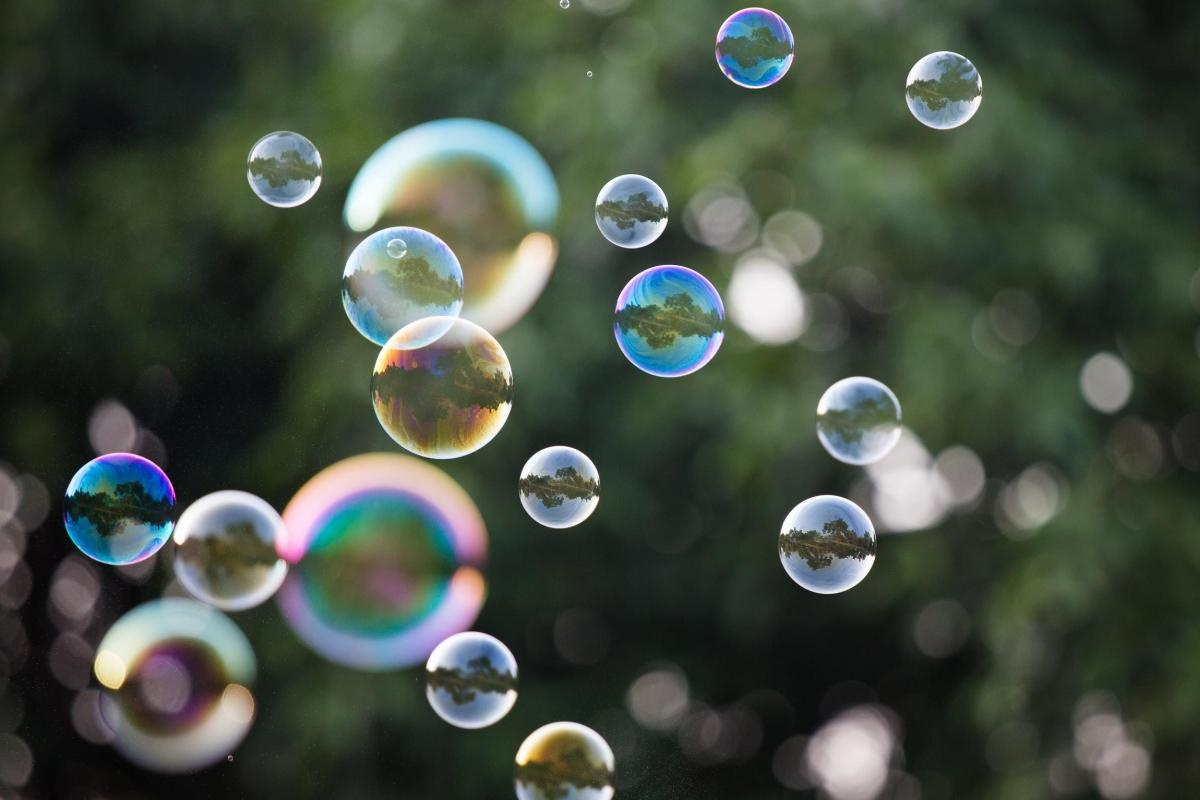
\includegraphics[width=.45\textwidth]{imagen_original.jpg}
    \caption{Imagen original utilizada para el análisis.}
    \label{fig:original}
\end{figure}

\FloatBarrier



\subsection{Conversión a Escala de Grises}
Para facilitar la detección de bordes, la imagen se convirtió a escala de grises, como se muestra en la Figura \ref{fig:grises}.


\FloatBarrier

\begin{figure}[h]
    \centering
    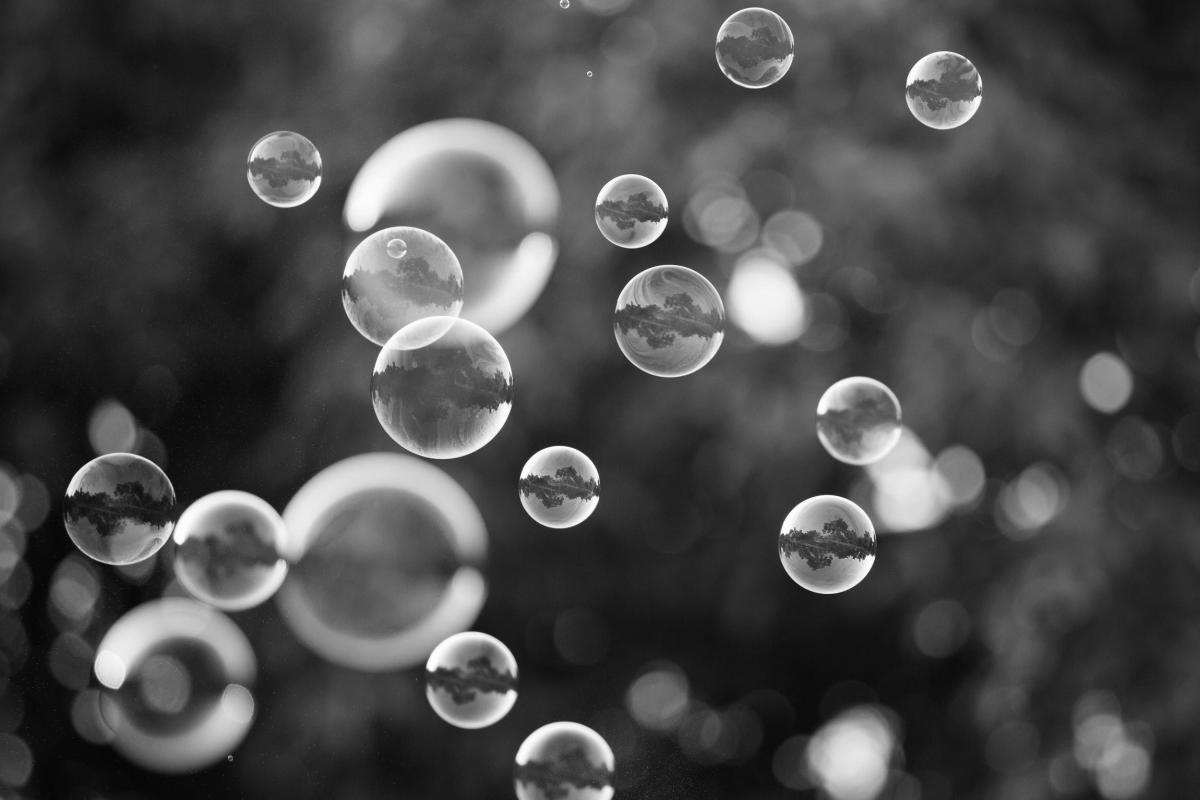
\includegraphics[width=0.45\textwidth]{imagen_grises.jpg}
    \caption{Imagen convertida a escala de grises.}
    \label{fig:grises}
\end{figure}

\FloatBarrier


\subsection{Aplicación de Desenfoque Gaussiano}
Se aplicó un filtro de desenfoque gaussiano para reducir el ruido, como se observa en la Figura \ref{fig:gauss}.

\FloatBarrier

\begin{figure}[h]
    \centering
    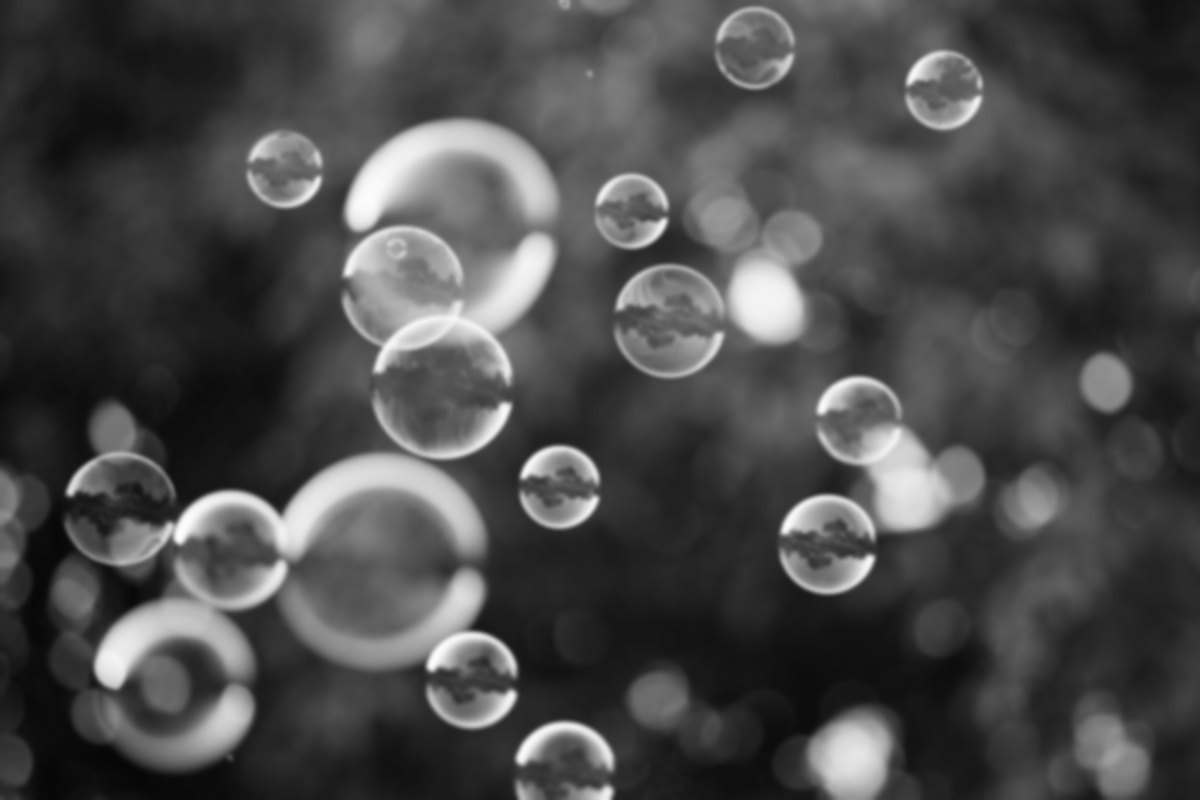
\includegraphics[width=0.45\textwidth]{imagen_gauss.jpg}
    \caption{Imagen después de aplicar desenfoque gaussiano.}
    \label{fig:gauss}
\end{figure}

\FloatBarrier


\section{Resultados}

La Figura \ref{fig:circulos} muestra los círculos detectados.

\FloatBarrier

\begin{figure}[h]
    \centering
    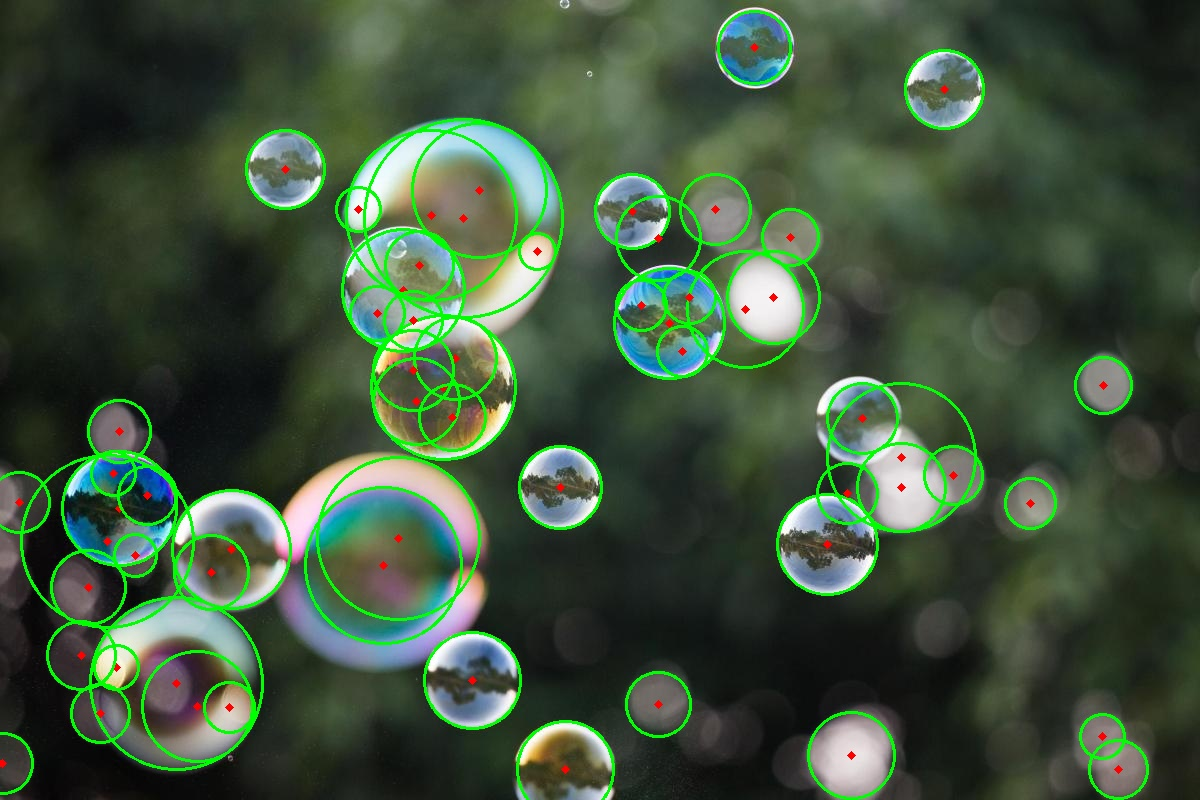
\includegraphics[width=0.45\textwidth]{imagen_circulos.jpg}
    \caption{Círculos detectados en la imagen mediante la Transformada de Hough.}
    \label{fig:circulos}
\end{figure}

\FloatBarrier


Tras ejecutar el código, se obtuvieron los siguientes resultados:
\begin{itemize}
    \item Se detectaron varios círculos en la imagen original.
    \item Algunos círculos fueron correctamente identificados, como el ojo de buey en la imagen.
    \item Se observaron \textbf{falsos positivos}, detectando círculos en áreas que no correspondían a objetos circulares.
    \item El desenfoque gaussiano ayudó a reducir ruido, pero pudo haber afectado la detección de círculos más pequeños.
    \item El histograma de la imagen en escala de grises mostró una distribución amplia de valores de intensidad, indicando que había variaciones de iluminación en la imagen.
\end{itemize}



\section{Conclusiones}

El presente estudio demostró que la Transformada de Hough es una herramienta efectiva para la detección de objetos circulares en imágenes digitales. Sin embargo, la precisión de la detección depende en gran medida del \textbf{preprocesamiento de la imagen} y de los \textbf{parámetros elegidos} en el algoritmo.

Se identificaron algunos \textbf{falsos positivos}, lo que sugiere que un refinamiento en la selección de bordes y en los valores de \texttt{param1} y \texttt{param2} podría mejorar los resultados.

Para trabajos futuros, se recomienda integrar técnicas de \textbf{aprendizaje profundo} y \textbf{segmentación avanzada} que permitan una detección más robusta y adaptable a diferentes condiciones de iluminación y ruido.

\section{Referencias}
\begin{itemize}
    \item Gonzalez, R. C., \& Woods, R. E. (2018). \textit{Digital Image Processing}. Pearson.
    \item Bradski, G., \& Kaehler, A. (2008). \textit{Learning OpenCV: Computer Vision with the OpenCV Library}. O'Reilly Media.
    \item OpenCV Documentation: \url{https://docs.opencv.org/}
    \item Hough Transform for Circle Detection: \url{https://en.wikipedia.org/wiki/Hough_transform}
\end{itemize}


\end{document}